\chapter{Universal software for machine learning in regulatory genomics}
\label{chap:chapter 1}

%%%%%%%%%%%%%%%%%%%%%%%%%%%%%%%%%%%%%%%%%%%%%%%%%%%%%%%%%%%%%%%%%%%%%%%%%%%%%%%%
\section{Abstract}
%%%%%%%%%%%%%%%%%%%%%%%%%%%%%%%%%%%%%%%%%%%%%%%%%%%%%%%%%%%%%%%%%%%%%%%%%%%%%%%%

Deep learning (DL) has become a popular tool to study cis-regulatory function. Yet, efforts to design software for DL analyses in regulatory genomics that are Findable, Accessible, Interoperable and Reusable (FAIR) have fallen short of fully meeting these criteria. Here, we present EUGENe (Elucidating the Utility of Genomic Elements with Neural Nets), a FAIR toolkit for the analysis of genomic sequences with DL. EUGENe consists of a set of modules and subpackages for executing the key functionality of a genomics DL workflow: 1) extracting, transforming and loading sequence data from many common file formats, 2) instantiating, initializing and training diverse model architectures, and 3) evaluating and interpreting model behavior. We designed EUGENe as a simple, flexible and extensible interface for streamlining and customizing end-to-end DL sequence analyses, and illustrate these principles through application of the toolkit to three predictive modeling tasks. We hope that EUGENe represents a springboard toward a collaborative ecosystem for DL applications in genomics research.

%%%%%%%%%%%%%%%%%%%%%%%%%%%%%%%%%%%%%%%%%%%%%%%%%%%%%%%%%%%%%%%%%%%%%%%%%%%%%%%%
\section{Main}
%%%%%%%%%%%%%%%%%%%%%%%%%%%%%%%%%%%%%%%%%%%%%%%%%%%%%%%%%%%%%%%%%%%%%%%%%%%%%%%%

Cracking the cis-regulatory code that governs gene expression remains a fundamental challenge in genomics research.

\begin{figure}[p]
    \centering
    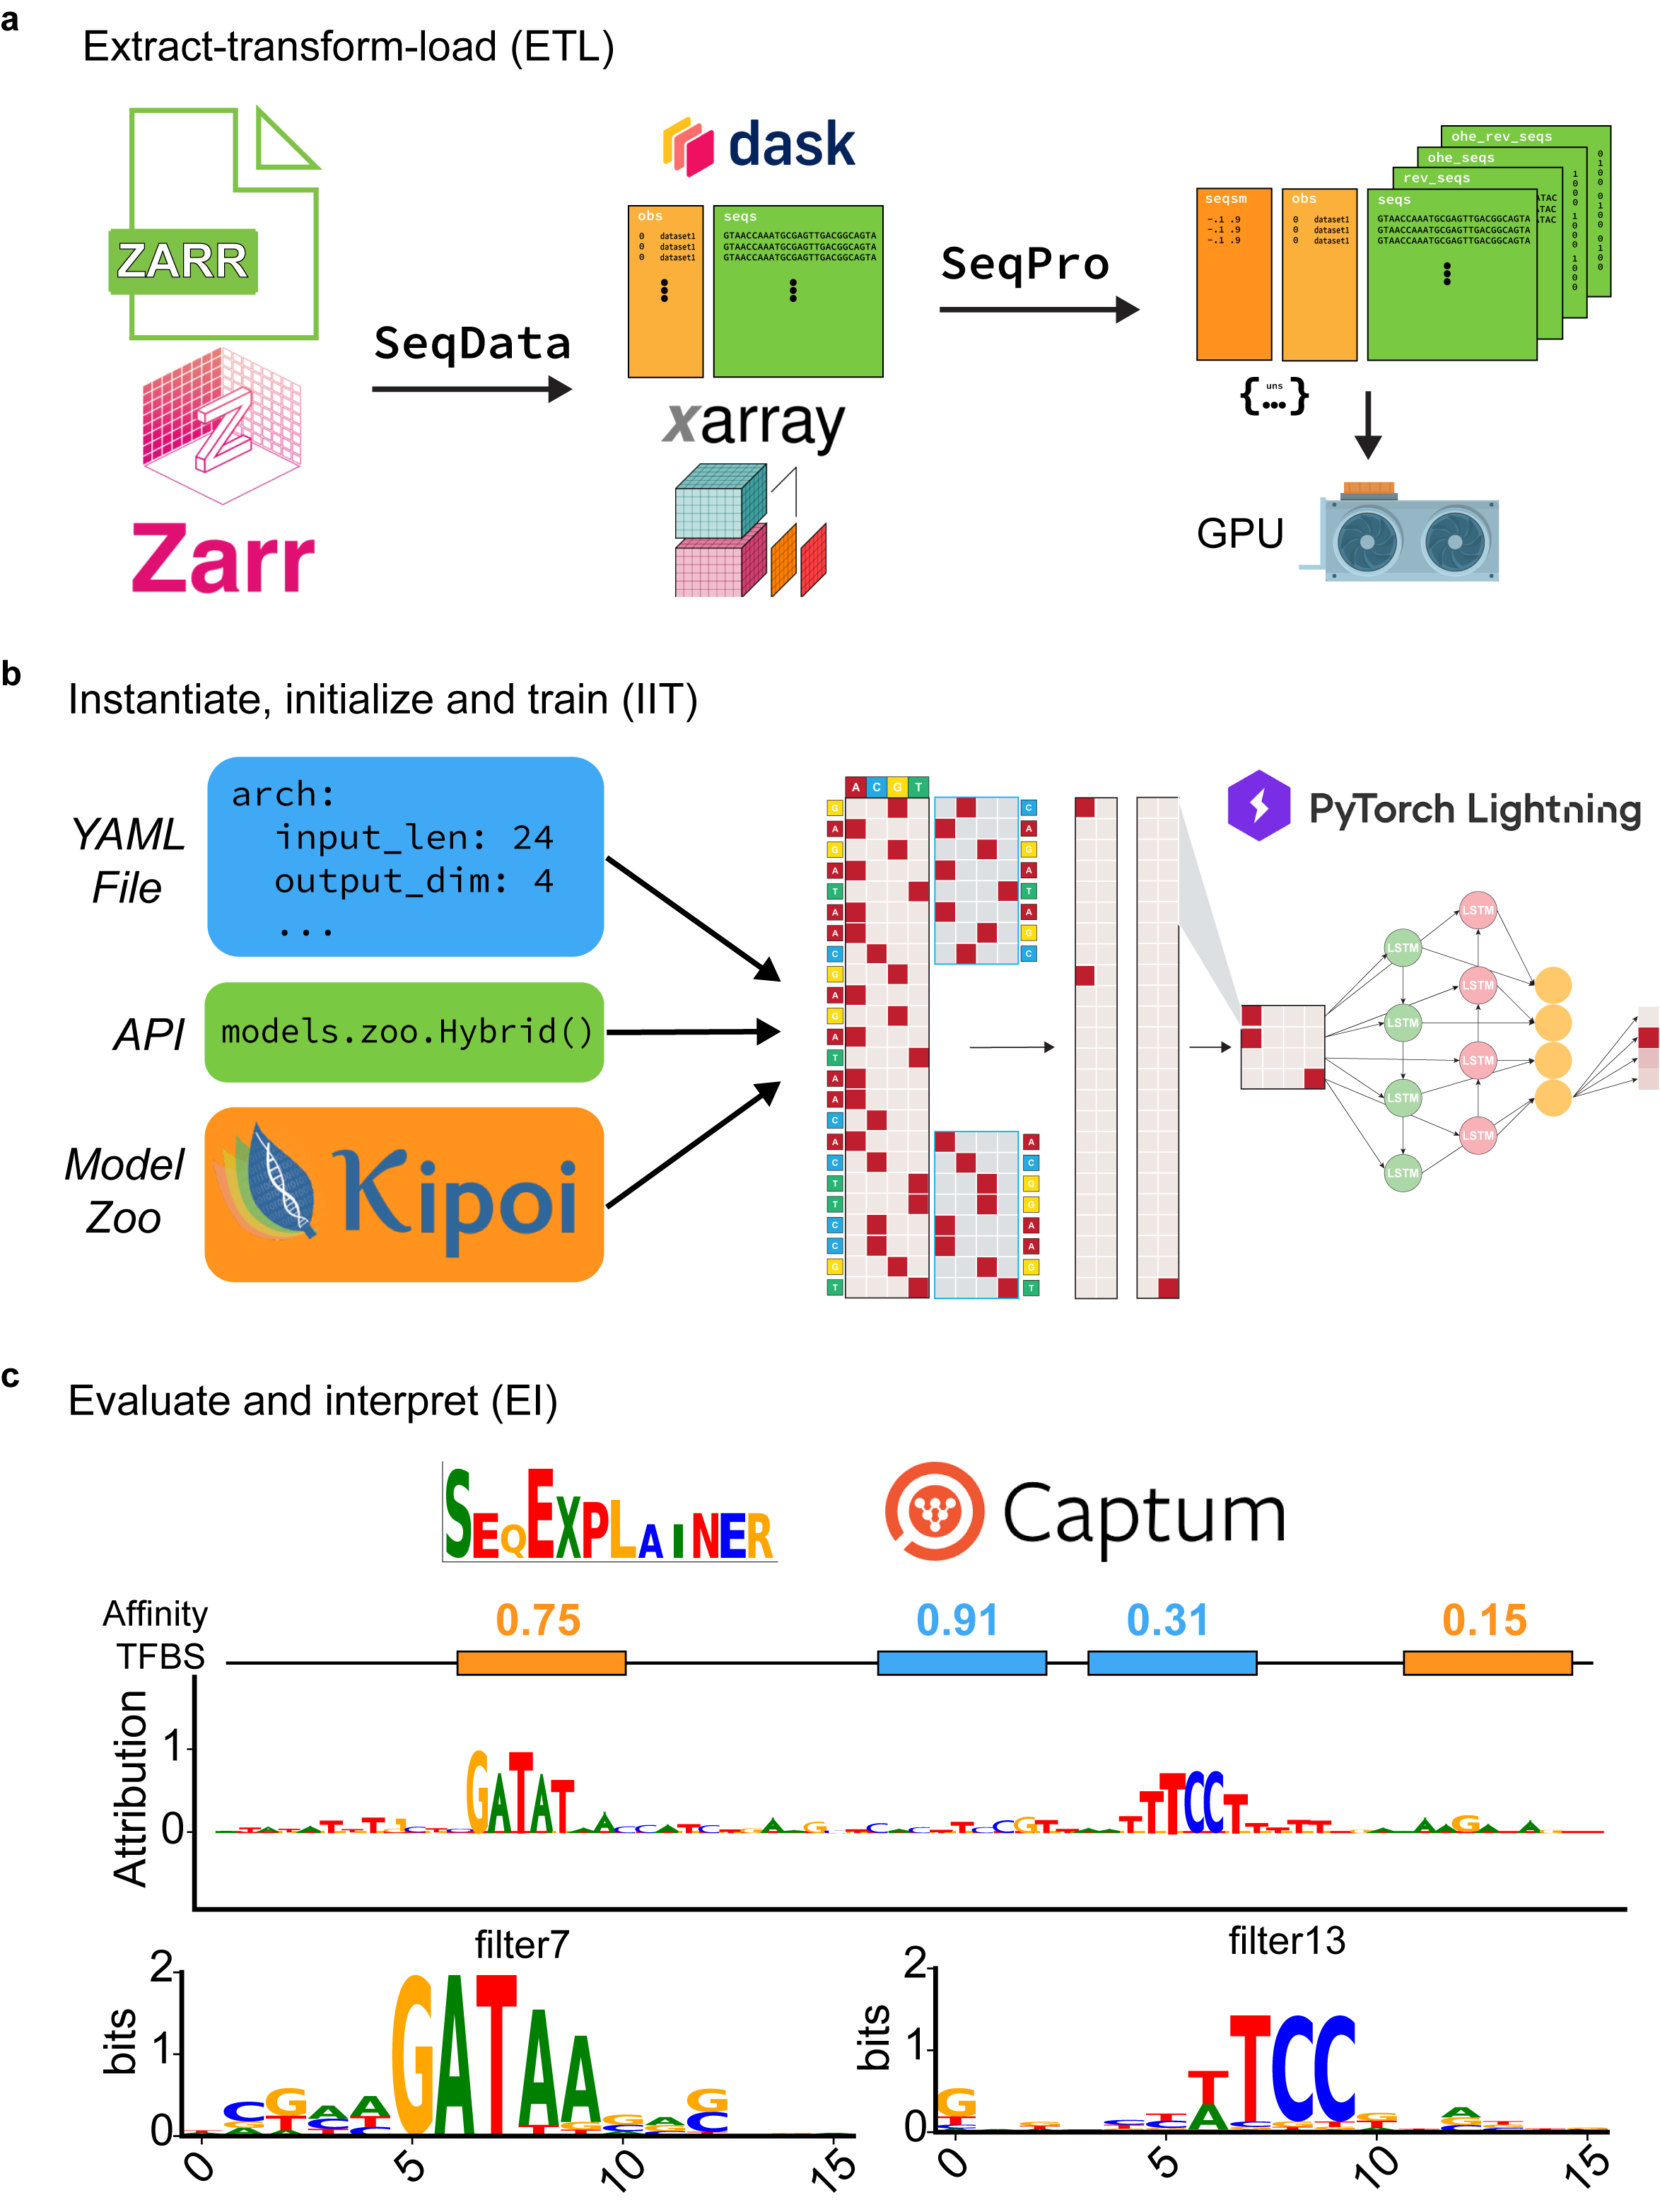
\includegraphics[width=0.9\textwidth, height=0.745\textheight]{1_figures-and-files/figure1.png}
    \caption[TODO]{TODO  
    }
    \label{fig:1 EUGENe Overview}
\end{figure}

\begin{figure}[p]
    \centering
    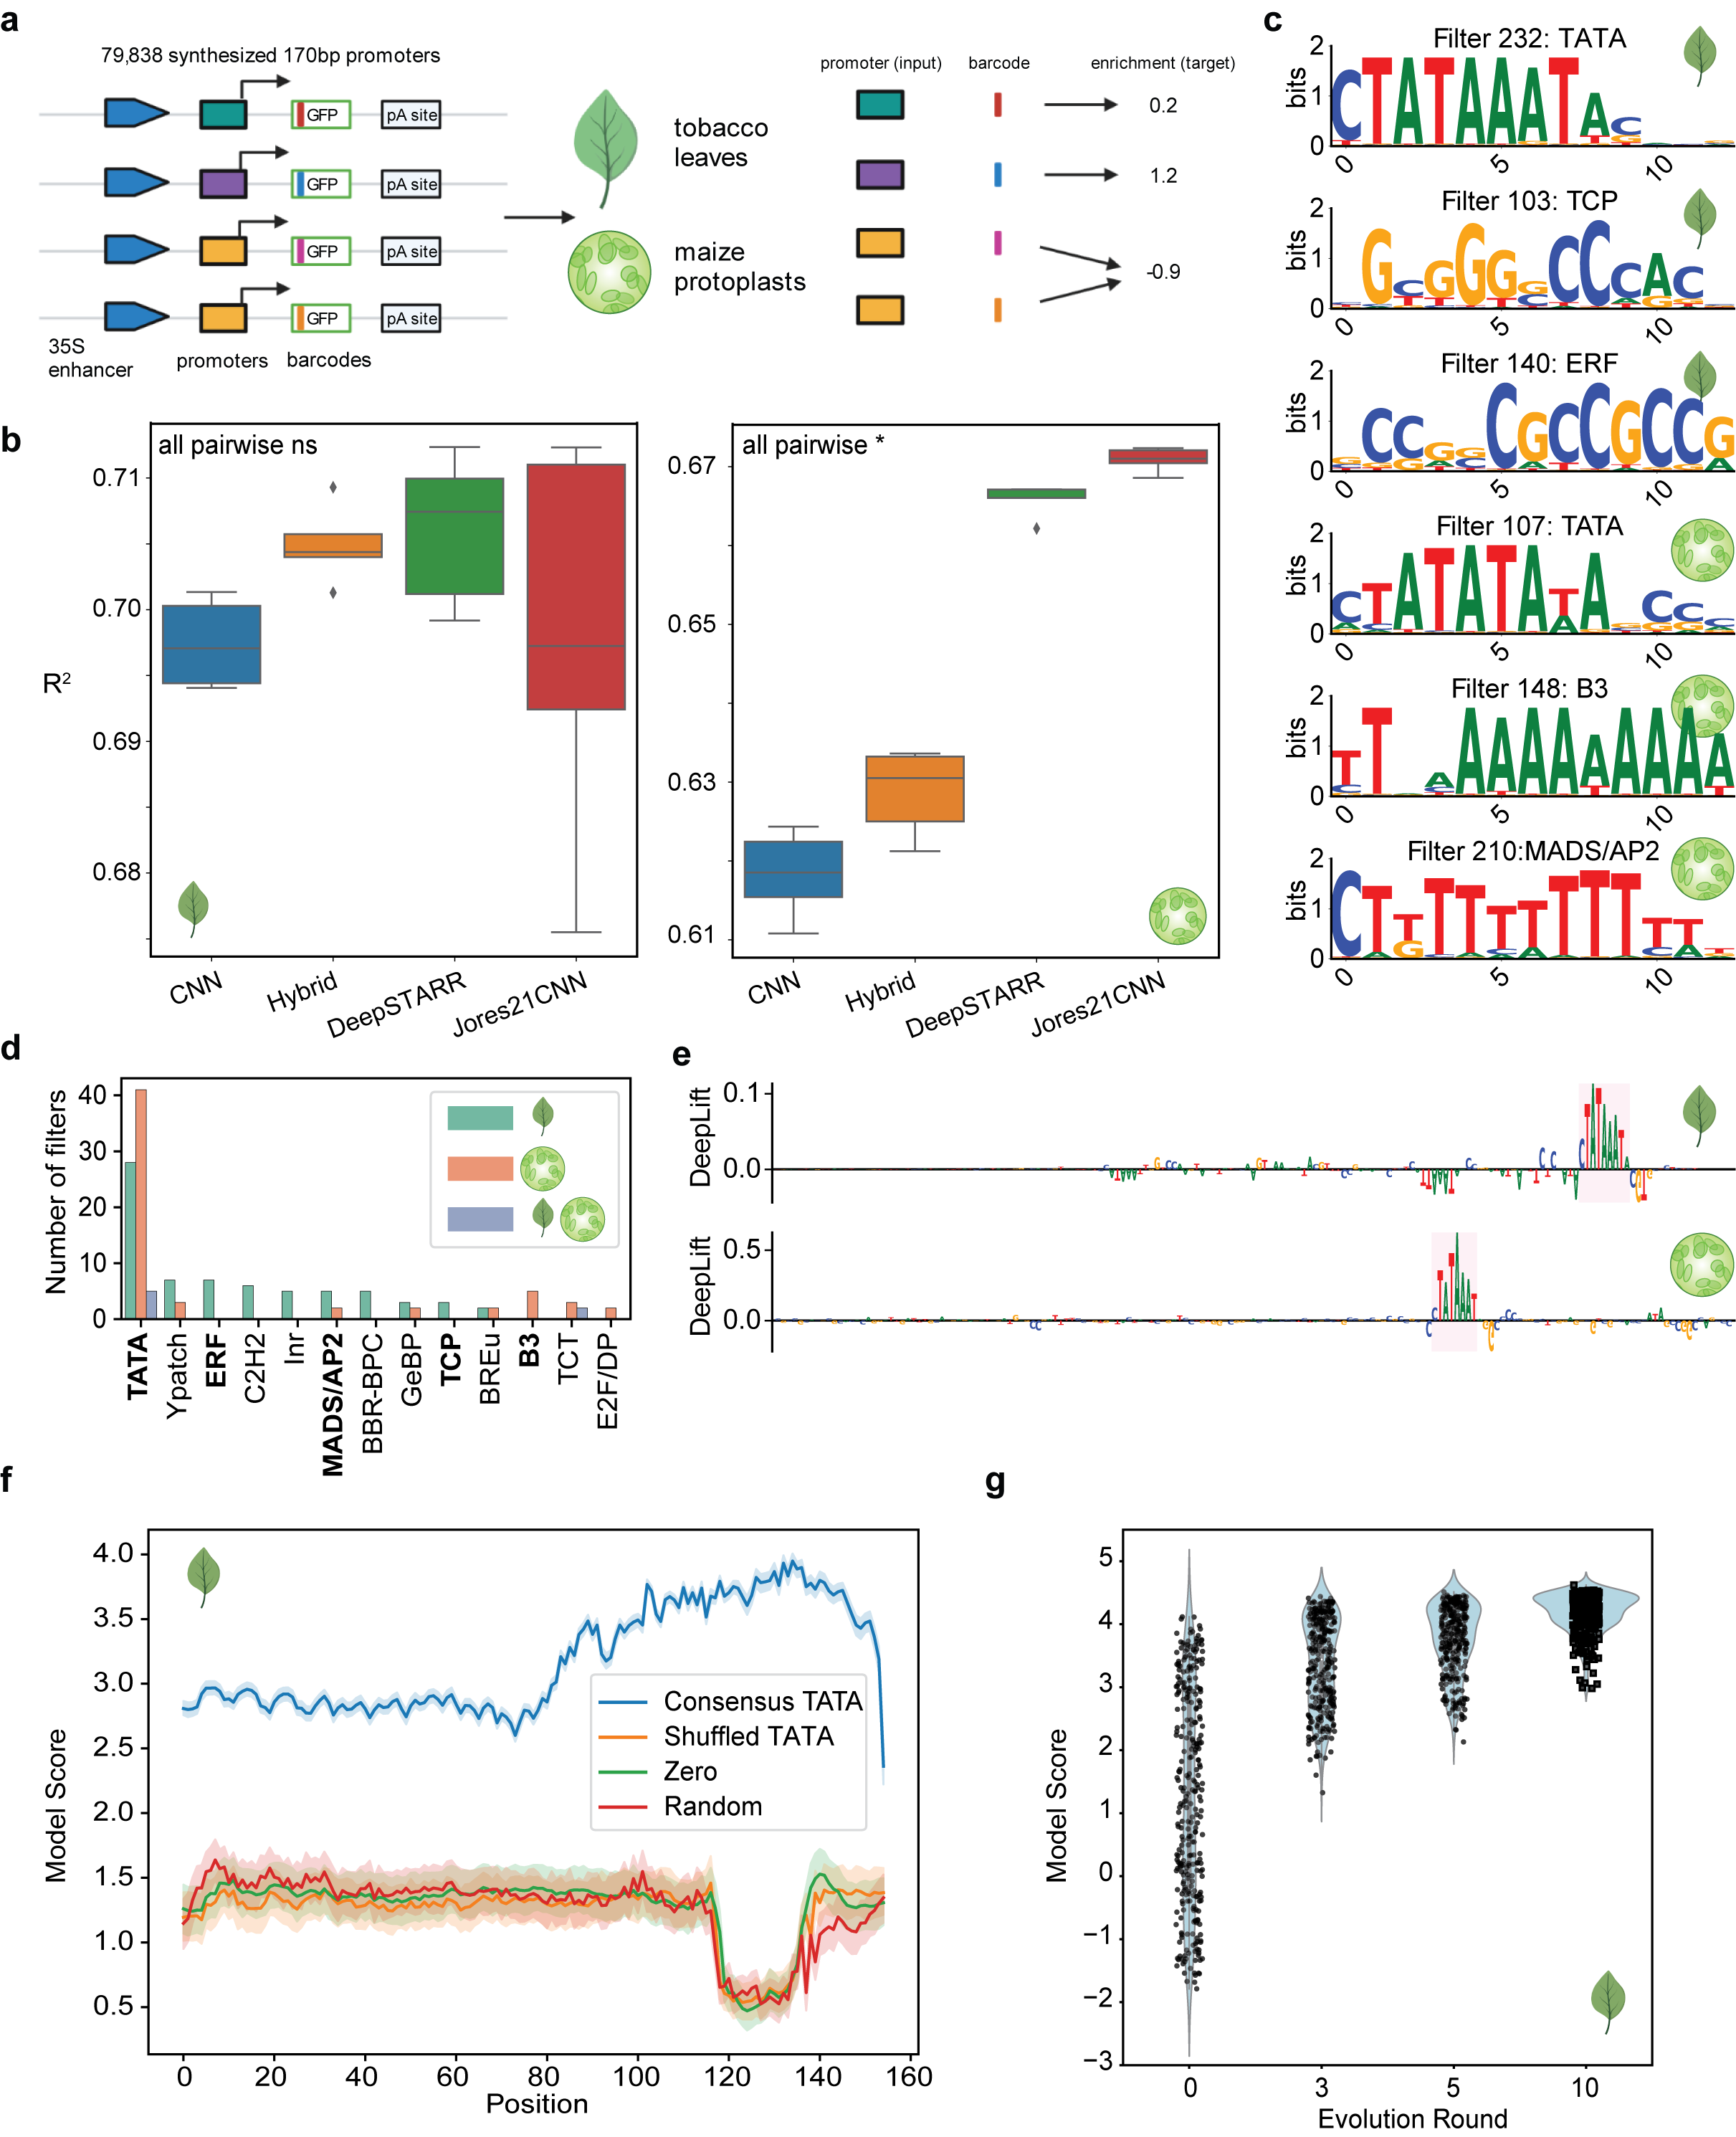
\includegraphics[width=0.9\textwidth, height=0.745\textheight]{1_figures-and-files/figure2.png}
    \caption[TODO]{TODO  
    }
    \label{fig:2}
\end{figure}

\begin{figure}[p]
    \centering
    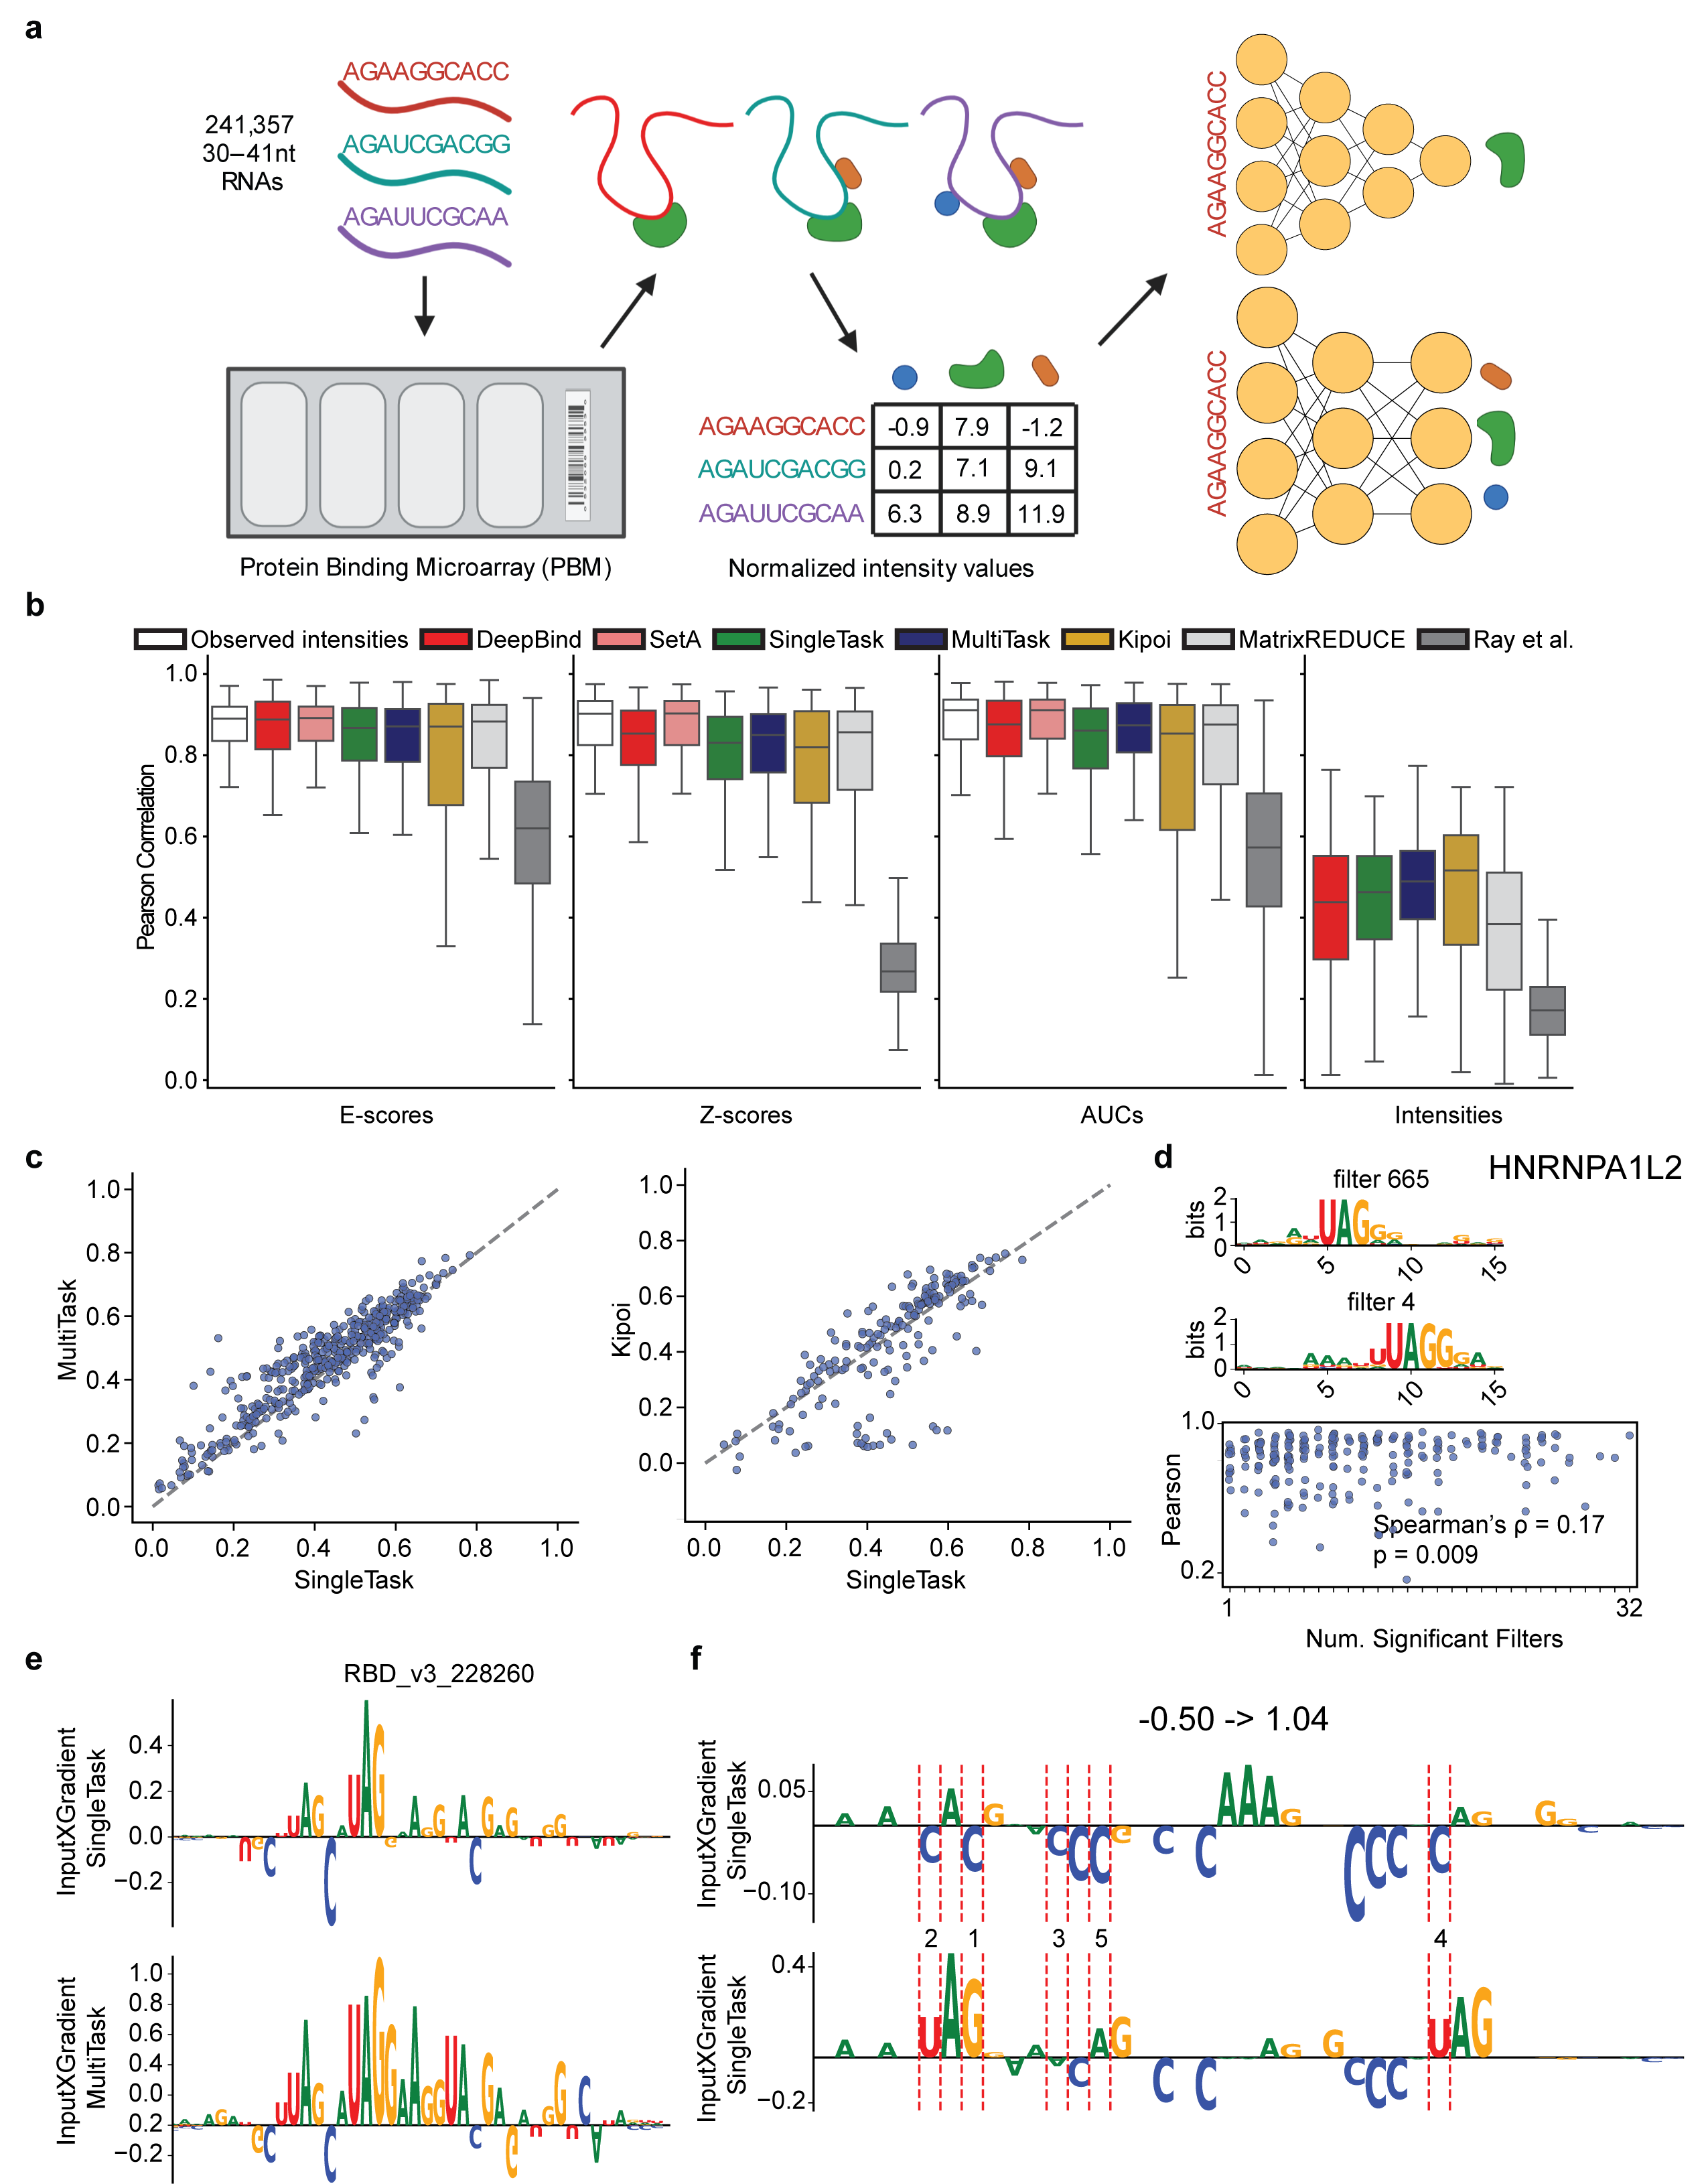
\includegraphics[width=0.9\textwidth, height=0.745\textheight]{1_figures-and-files/extended_data_figure1.png}
    \caption[TODO]{TODO  
    }
    \label{fig:3 Extended Data Figure 1}
\end{figure}

\begin{figure}[p]
    \centering
    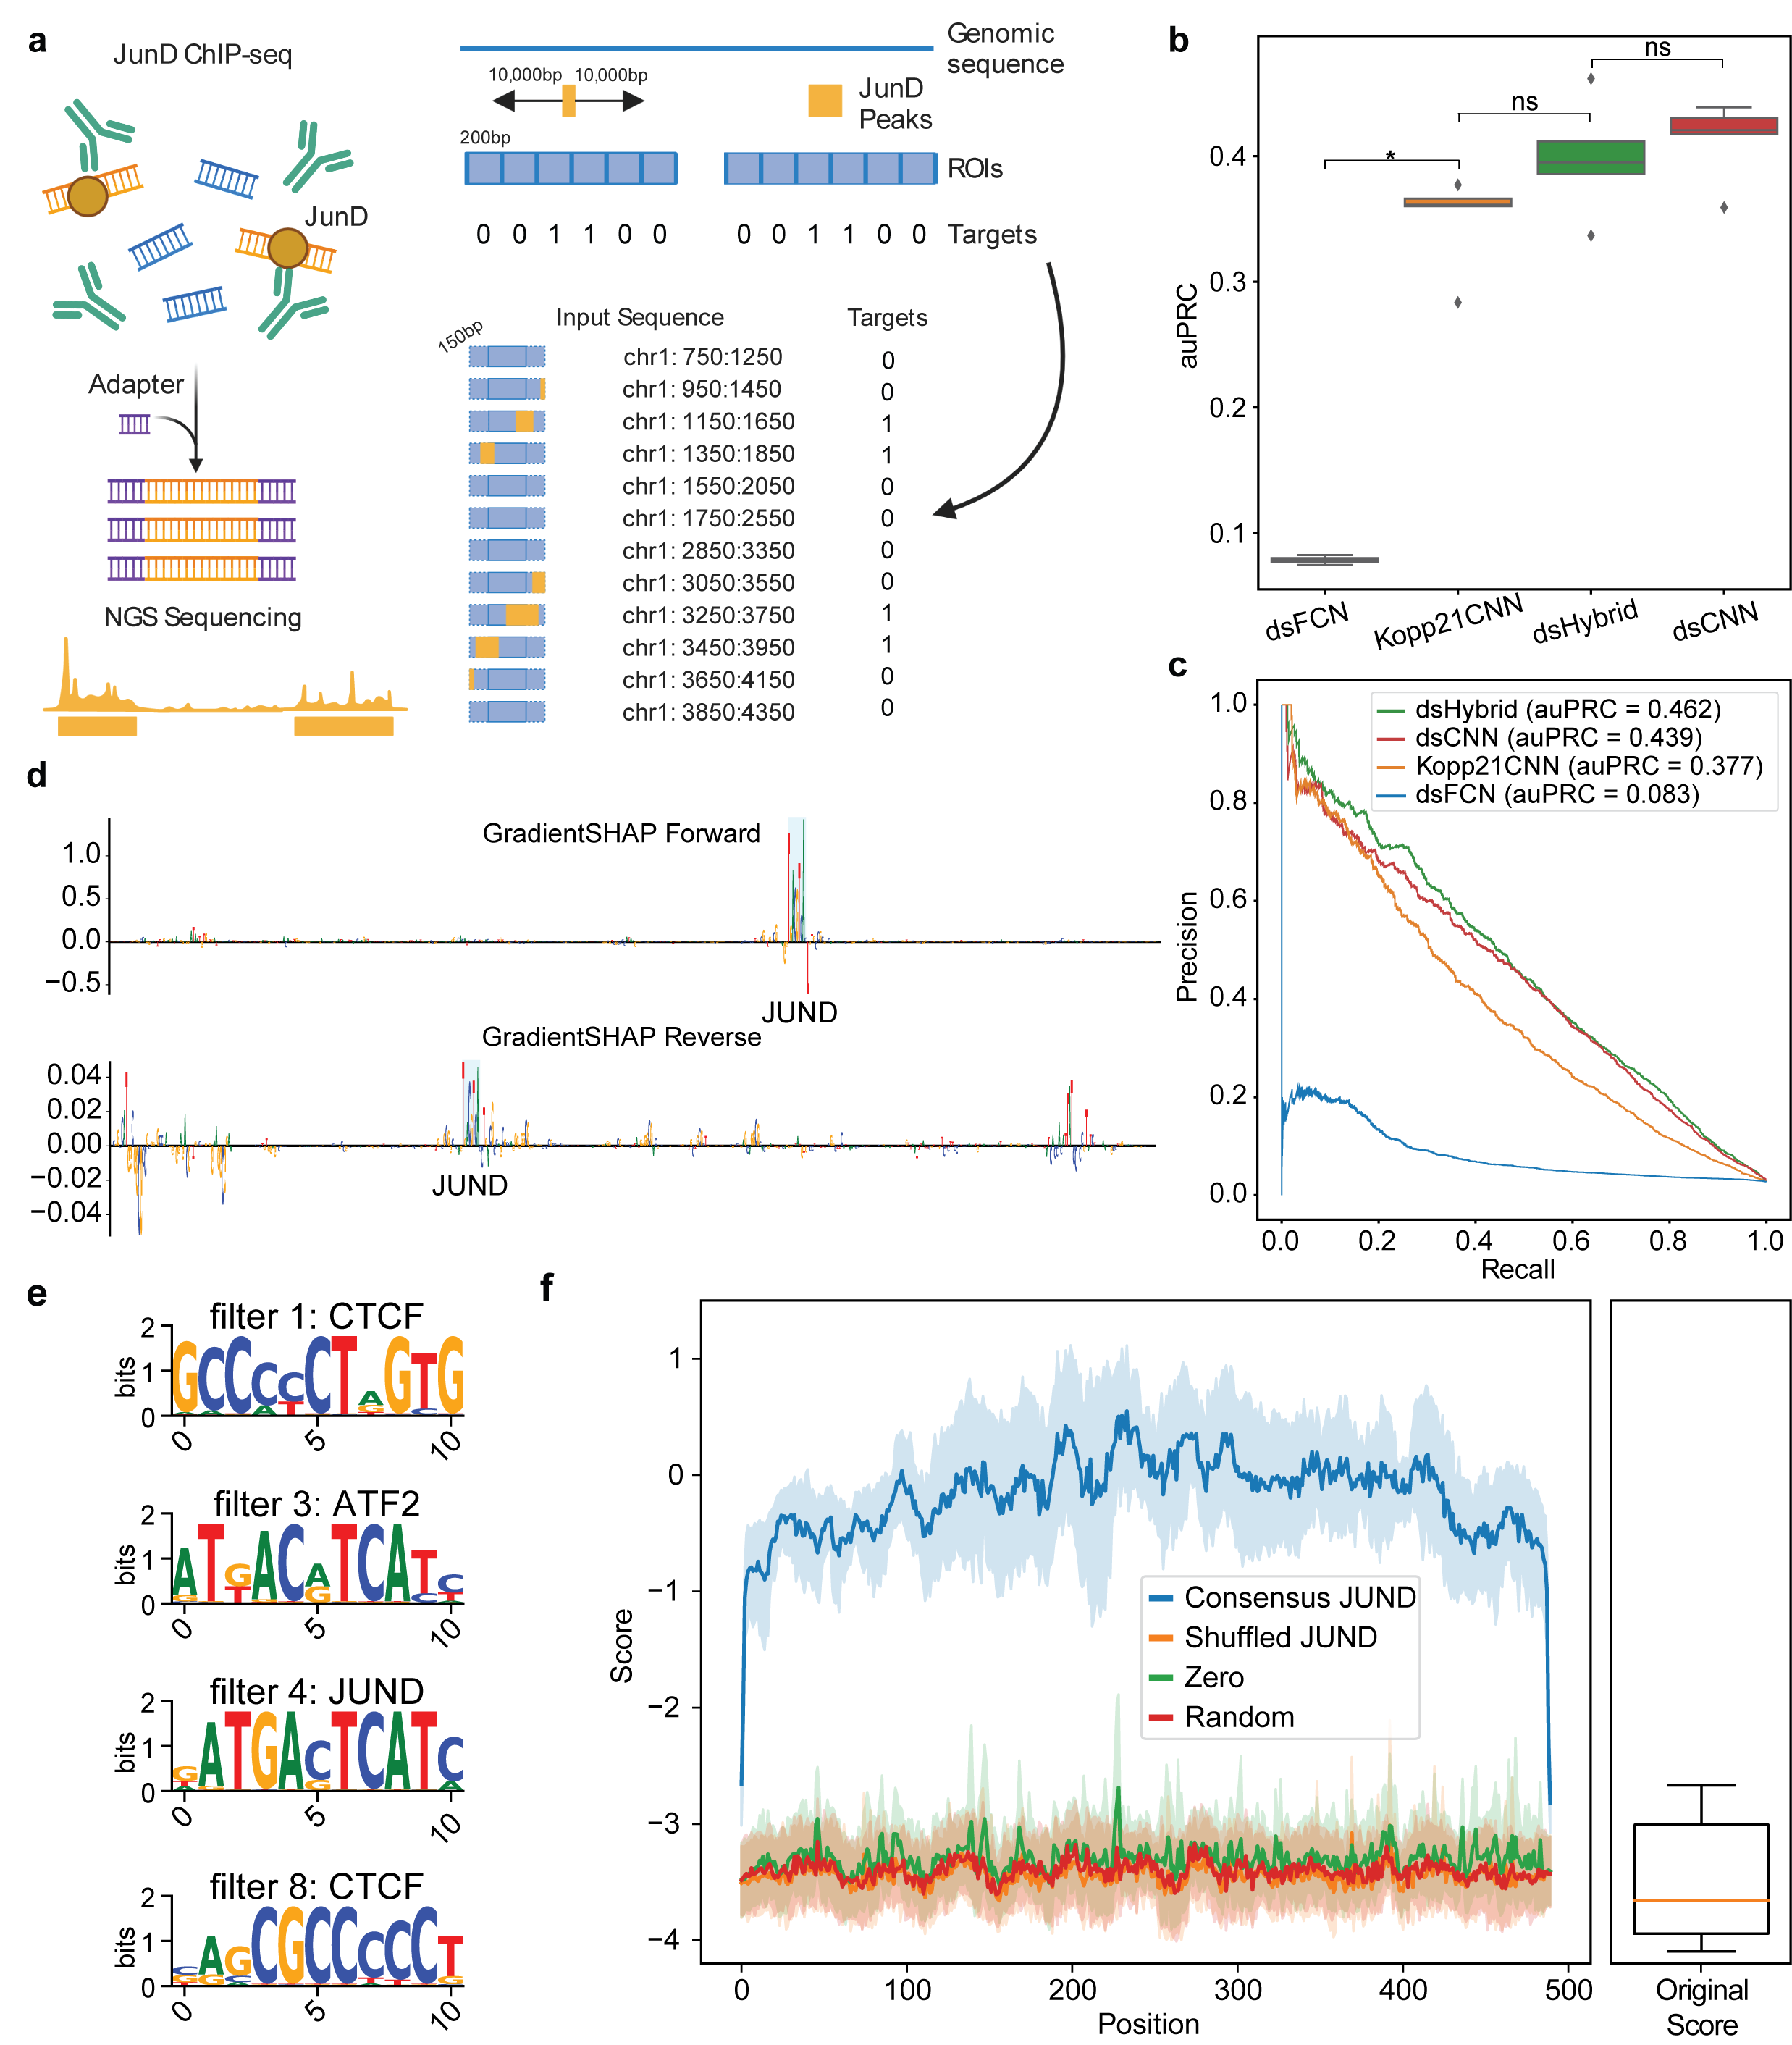
\includegraphics[width=0.9\textwidth, height=0.745\textheight]{1_figures-and-files/extended_data_figure2.png}
    \caption[TODO]{TODO  
    }
    \label{fig:4 Extended Data Figure 2}
\end{figure}

\begin{figure}[p]
    \centering
    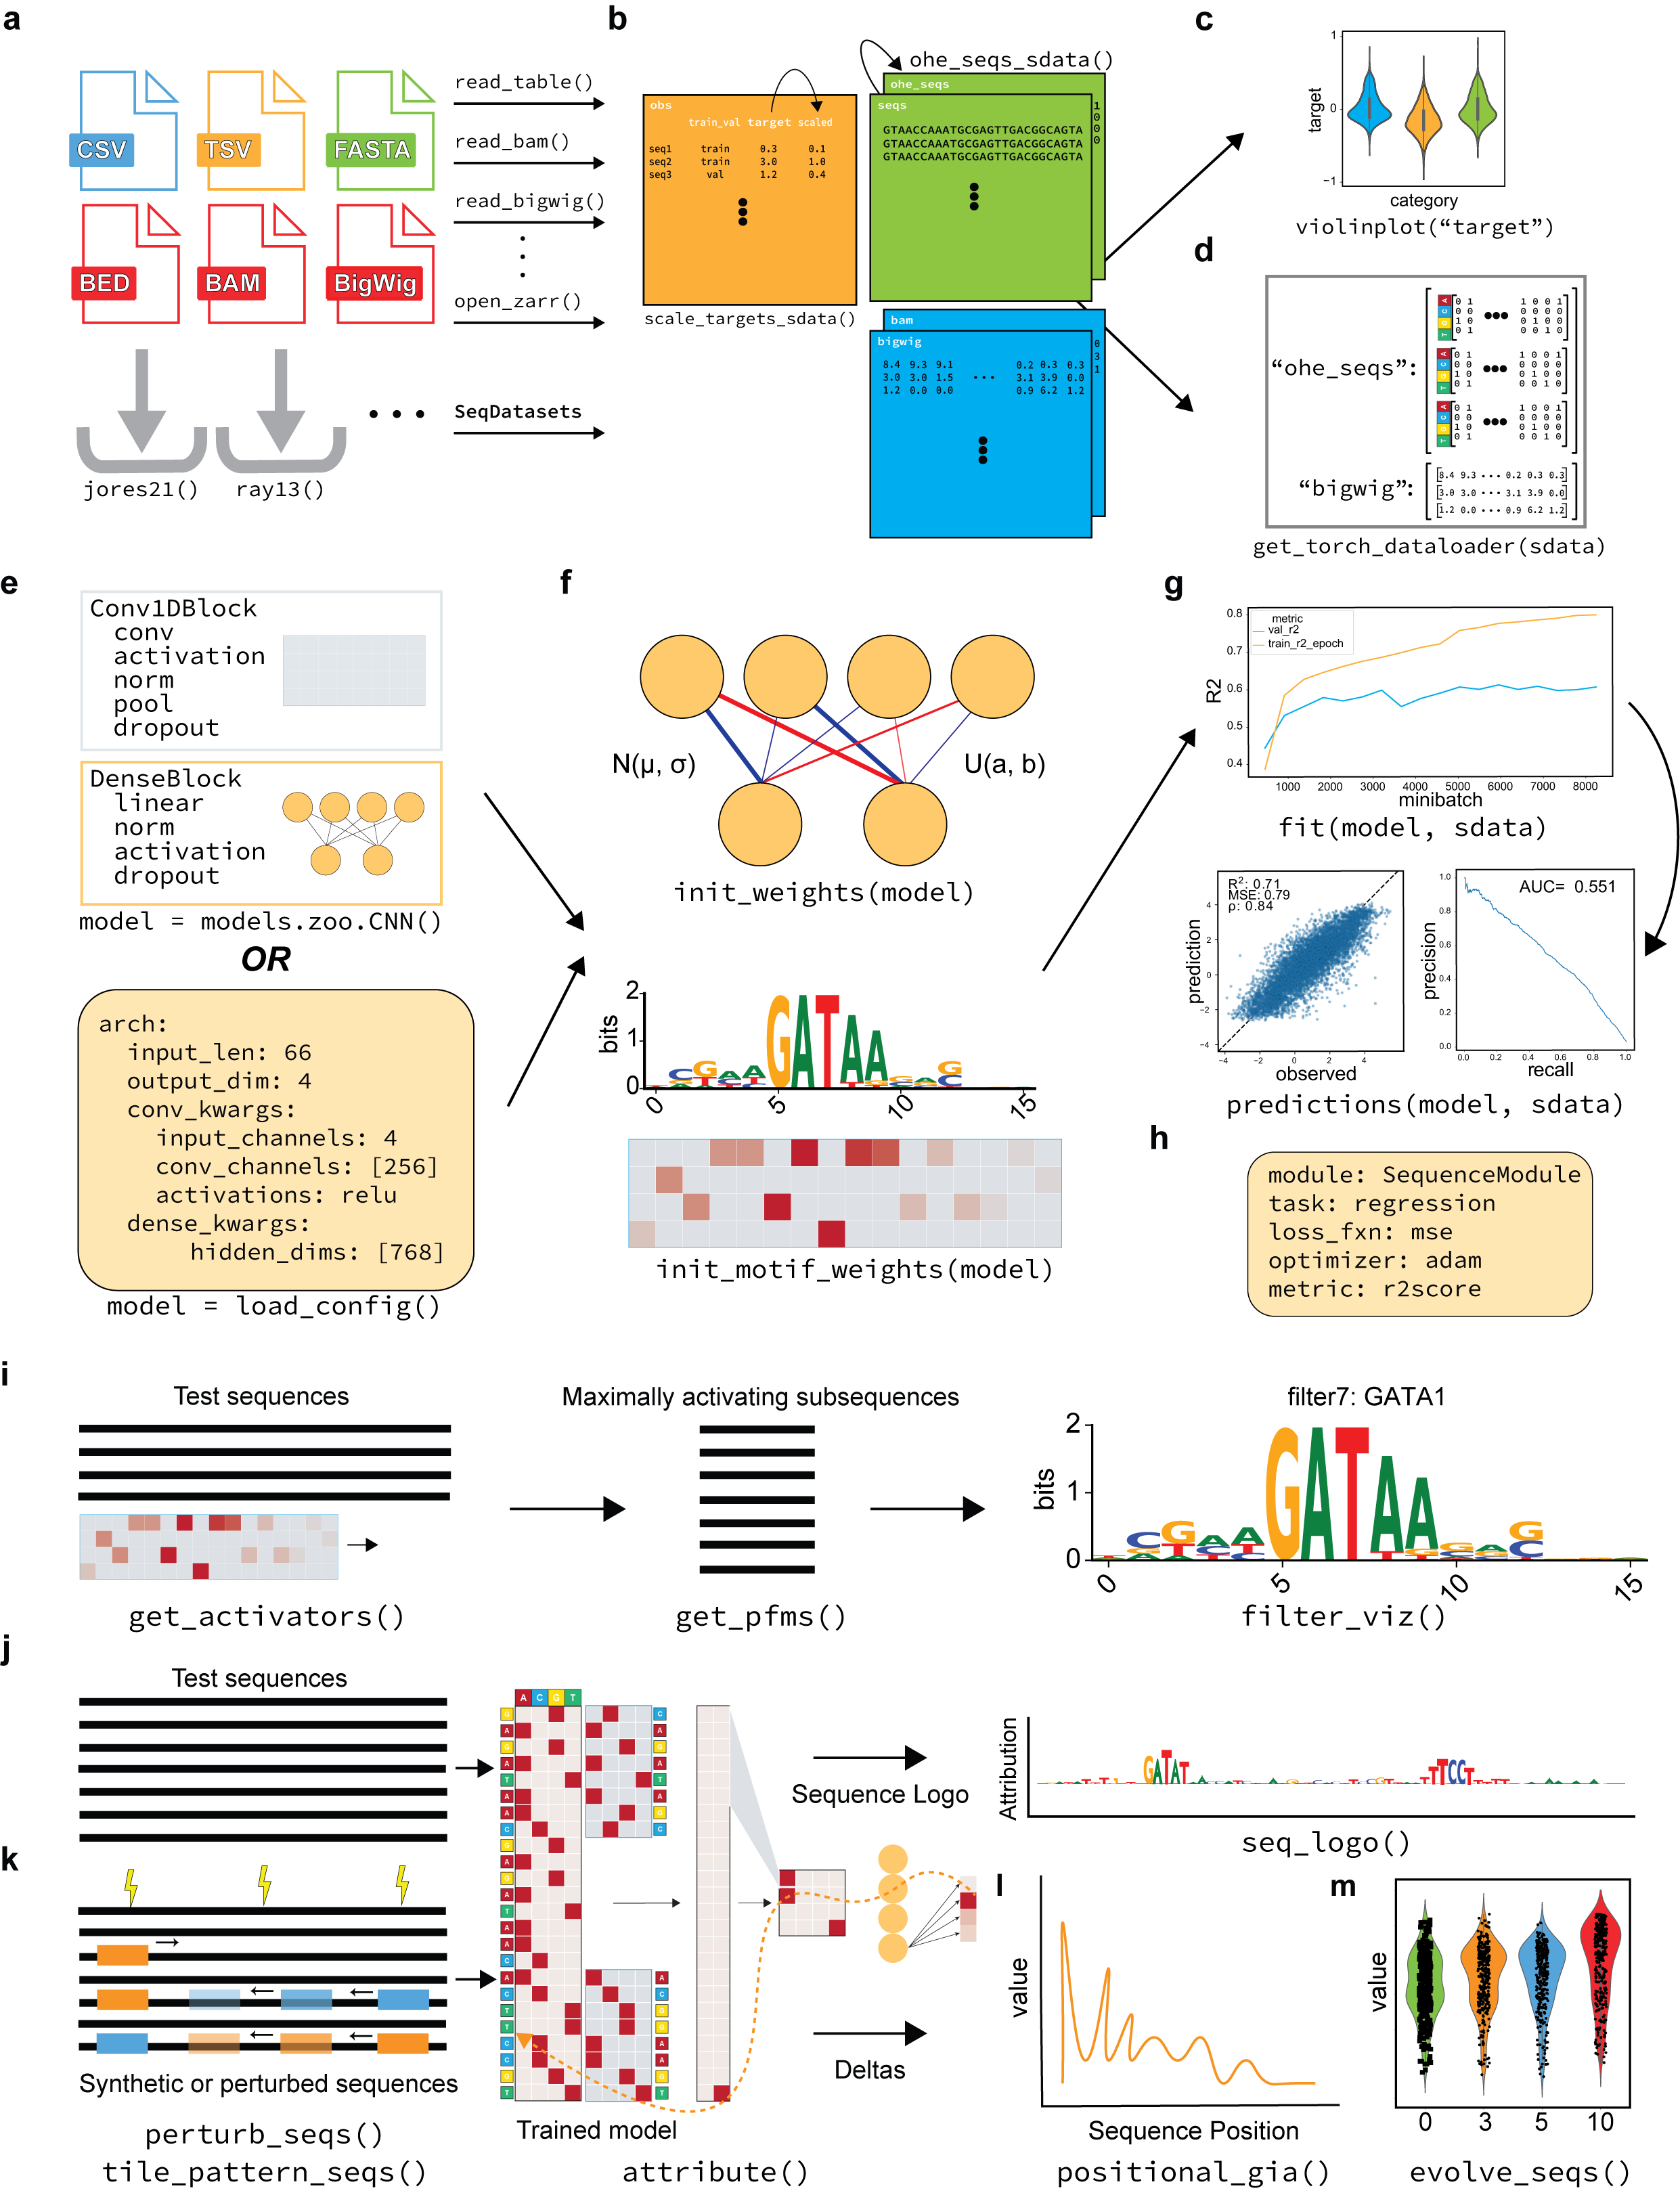
\includegraphics[width=0.9\textwidth, height=0.745\textheight]{1_figures-and-files/extended_data_figure3.png}
    \caption[TODO]{TODO  
    }
    \label{fig:5 Extended Data Figure 3}
\end{figure}

%%%%%%%%%%%%%%%%%%%%%%%%%%%%%%%%%%%%%%%%%%%%%%%%%%%%%%%%%%%%%%%%%%%%%%%%%%%%%%%%
\section{Methods}
%%%%%%%%%%%%%%%%%%%%%%%%%%%%%%%%%%%%%%%%%%%%%%%%%%%%%%%%%%%%%%%%%%%%%%%%%%%%%%%%

\subsection{The EUGENe workflow}

\subsubsection{Data extraction, transformation and loading with SeqData}

\subsubsection{Model training with PyTorch and PyTorch Lightning}

\subsubsection{Model interpretation with SeqExplainer}

\subsection{Analysis of plant promoter data}

\subsubsection{Data acquisition and preprocessing}

\subsubsection{Model initialization and training}

\subsubsection{Model evaluation and interpretation}

\subsection{Analysis of RNA binding data}

\subsubsection{Data acquisition and preprocessing}

\subsubsection{Model initialization and training}

\subsubsection{Model evaluation}

\subsubsection{Model interpretation}

\subsection{Analysis of JunD binding data}

\subsubsection{Data acquisition and preprocessing}

\subsubsection{Model initialization and training}

\subsubsection{Model evaluation and interpretation}

\subsection{Data visualization software}

\subsection{Statistical methods}

%%%%%%%%%%%%%%%%%%%%%%%%%%%%%%%%%%%%%%%%%%%%%%%%%%%%%%%%%%%%%%%%%%%%%%%%%%%%%%%%
\section{Data availability}
%%%%%%%%%%%%%%%%%%%%%%%%%%%%%%%%%%%%%%%%%%%%%%%%%%%%%%%%%%%%%%%%%%%%%%%%%%%%%%%%

%%%%%%%%%%%%%%%%%%%%%%%%%%%%%%%%%%%%%%%%%%%%%%%%%%%%%%%%%%%%%%%%%%%%%%%%%%%%%%%%
\section{Code availability}
%%%%%%%%%%%%%%%%%%%%%%%%%%%%%%%%%%%%%%%%%%%%%%%%%%%%%%%%%%%%%%%%%%%%%%%%%%%%%%%%

%%%%%%%%%%%%%%%%%%%%%%%%%%%%%%%%%%%%%%%%%%%%%%%%%%%%%%%%%%%%%%%%%%%%%%%%%%%%%%%%
\section{Acknowledgements}
%%%%%%%%%%%%%%%%%%%%%%%%%%%%%%%%%%%%%%%%%%%%%%%%%%%%%%%%%%%%%%%%%%%%%%%%%%%%%%%%

%%%%%%%%%%%%%%%%%%%%%%%%%%%%%%%%%%%%%%%%%%%%%%%%%%%%%%%%%%%%%%%%%%%%%%%%%%%%%%%%
\section{Author information}
%%%%%%%%%%%%%%%%%%%%%%%%%%%%%%%%%%%%%%%%%%%%%%%%%%%%%%%%%%%%%%%%%%%%%%%%%%%%%%%%

%%%%%%%%%%%%%%%%%%%%%%%%%%%%%%%%%%%%%%%%%%%%%%%%%%%%%%%%%%%%%%%%%%%%%%%%%%%%%%%%
\section{Ethics declarations}
%%%%%%%%%%%%%%%%%%%%%%%%%%%%%%%%%%%%%%%%%%%%%%%%%%%%%%%%%%%%%%%%%%%%%%%%%%%%%%%%

\subsection{Competing interests}
